\documentclass[a4paper]{scrartcl}

\usepackage{float}
\usepackage{tikz}
\usetikzlibrary{arrows,automata}
\usepackage{pgf}
\usepackage[utf8]{inputenc} % this is needed for umlauts
\usepackage[ngerman]{babel} % this is needed for umlauts
\usepackage[T1]{fontenc}    % this is needed for correct output of umlauts in pd
\usepackage{amssymb}
\usepackage{amsmath}
\usepackage{mathrsfs}
\usepackage{dsfont}
\usepackage{graphicx}
\usepackage{fancyhdr}
\usepackage{lastpage}
\usepackage{imakeidx}
\setlength{\parskip}{\medskipamount}
\setlength{\parindent}{0pt}
\usepackage{enumitem}
\usepackage{hyperref}
\usepackage{verbatim}

%%%%%%%%%%%%%%%%%%%%%%%%
% Kopf- und Fusszeilen %
%%%%%%%%%%%%%%%%%%%%%%%%
\pagestyle{fancy}
\lhead{
        Maximilian Roth
}
\chead{Logik-Tutorat Lösungen Blatt 5\\}
\rhead{
        \today{} \\
        Seite \thepage{} von \pageref{LastPage}\\
        
}
\lfoot{}
\cfoot{}
\rfoot{} 

%%%%%%%%%%%%%%%%%%%%%%%%
% Anfang des Dokuments %
%%%%%%%%%%%%%%%%%%%%%%%%

\begin{document}
\section*{Disclaimer}%{{{
\label{sec:disclaimer}
Auch in diesem Dokument können sich Fehler befinden!\\
Sie sind nicht die Musterlösung der Aufgaben, sondern selbst erstellte Lösungen.\\

Als generelle Lektüre kann ich nur das Skript von Markus Junker aus dem WS 17/18 empfehlen:\\
\url{http://home.mathematik.uni-freiburg.de/junker/skripte/InfoLogik.pdf}\\
Hier ist vieles sehr genau und verständlich erklärt.%}}}

\section*{}%{{{
\label{sec:aufgabe_1}

    \begin{figure}[H]
        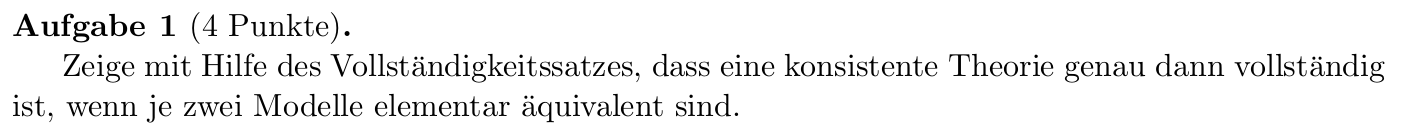
\includegraphics[scale=0.3]{./A-1.png}
        \label{fig:}
    \end{figure}

    Sei T konsistente Theorie, $\mathcal{A},\mathcal{B} \mathscr{L}$-Strukturen, $\mathcal{A} \vDash T, \mathcal{B} \vDash T$\\
    \\\underline{ZZ:} T vollständig $\Leftrightarrow \mathcal{A} \equiv \mathcal{B}$\\
    \\\underline{Beweis:}\\

    \begin{itemize}
        \item T vollständig $\Rightarrow \mathcal{A} \equiv \mathcal{B}$\\
            T vollständig und $\chi \mathscr{L}$-Aussage\\
            Gilt nun $\mathcal{A} \vDash \chi$:\\
            \\$\mathcal{A} \vDash \chi\\
            \overset{\mathcal{A}\vDash T}{\Leftrightarrow} T \vdash \chi\\
            \overset{B \vDash T}{\Leftrightarrow}\mathcal{B} \vDash \chi\\
            \overset{\text{B analog}}{\Rightarrow} \mathcal{A} \equiv \mathcal{B}$\\
        
        \item $\mathcal{A} \equiv \mathcal{B} \Rightarrow$ T vollständig\\
            Sei $\chi \mathscr{L}$-Aussage\\
            \begin{itemize}
                \item $T \nvdash \chi\\
                    \overset{\mathcal{A} \vDash T}{\Rightarrow} \mathcal{A} \nvdash \chi\\
                    \overset{\chi \mathscr{L}\text{-Auss.}}{\Rightarrow} \mathcal{A} \vdash \neg \chi$\\

                \item $T \vdash \chi\\
                    \overset{\mathcal{B} \vDash T}{\Rightarrow} \mathcal{B} \vdash \chi$\\
            \end{itemize}

            Da $\mathcal{A} \equiv \mathcal{B}$ kann nicht gleichzeitig $T \vdash \chi$ und $T \nvdash \chi$ gelten.\\
            $\Rightarrow$ T vollständig\\

    \end{itemize}
%}}}

\section*{}%{{{
\label{sec:aufgabe_2}

    \begin{figure}[H]
        \centering
        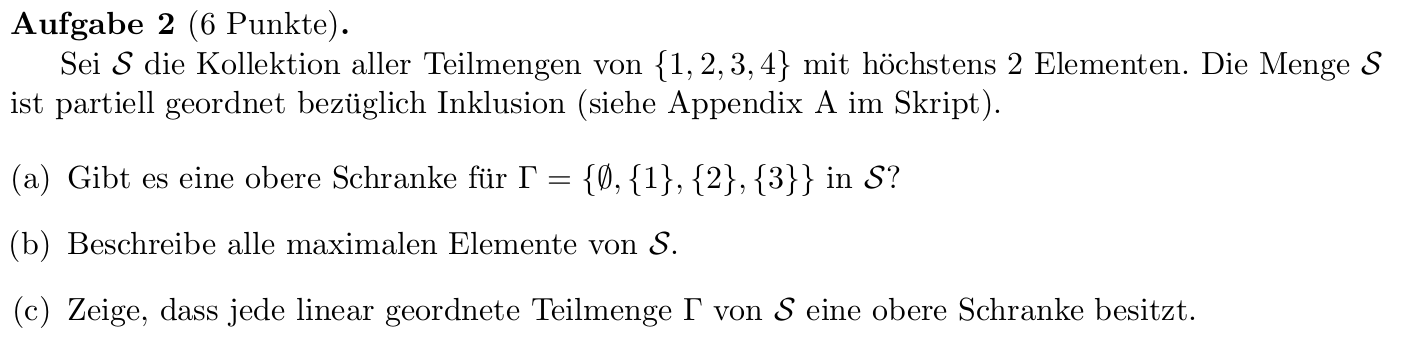
\includegraphics[scale=0.3]{./A-2.png}
        \label{fig:}
    \end{figure}

    \begin{itemize}
        \item a)\\
            \underline{ZZ:} Es gibt keine obere Schranke B für $\Gamma$\\
            \underline{Beweis:}\\
                B müsste Obermenge von \{\},\{1\},\{2\} und \{3\} sein und damit mindestens 1,2,3 enthalten.\\
                $\Rightarrow |B| \geq 3$ Damit ist B nicht in S. Widerspruch!\\
                \\$\Rightarrow$ Es gibt keine obere Schranke für $\Gamma$\\

        \item b)\\
            Die maximalen Elemente müssen 2-elementige Mengen sein.\\
            Wären sie kleiner, wären sie selbst Teilmenge einer solchen.\\
            Wären sie größer, wären sie nicht mehr in S.\\
            Damit sind alle 2-elementigen Teilmengen maximale Elemente.\\

\newpage

        \item c)\\
            $\mathcal{S}$ sind alle maximal 2-Elementigen Teilmengen von \{1,2,3,4\}\\
            $\Rightarrow \Gamma$ sind ebenfalls solche, aber nicht alle.\\
            $\Rightarrow \forall A \in \Gamma$ ist Teilmenge von \{1,2,3,4\}\\
            \\$\bigcup_{A \in \Gamma}$ wäre obere Schranke für $\Gamma$, da es alle Elemente dessen enthält.\\
            \\Aber liegt $\bigcup_{A \in \Gamma}$ auch in $\mathcal{S}$?\\
            \\Wir zeigen, dass $\bigcup_{A \in \Gamma}$ maximal 2-Elementige Teilmenge von \{1,2,3,4\} ist.\\
            Das ist dann der Fall, wenn für $A,B \in \Gamma: (A \cup B) \in \mathcal{S}$\\
            \\Da $\mathcal{S}$ linear geordnet ist können wir unterteilen in:\\
            \begin{itemize}
                \item $A \subset B \Rightarrow A \cup B = B \in \mathcal{S}$\\
                \item $A = B \Rightarrow A \cup B = A \in \mathcal{S}$\\
                \item $B \subset A \Rightarrow A \cup B = A \in \mathcal{S}$\\
            \end{itemize}
            Damit folgt, dass $\bigcup_{A \in \Gamma} \in \mathcal{S}$ und damit obere Schranke ist.\\
            





    \end{itemize}

%}}}

\section*{}%{{{
\label{sec:aufgabe_3}

    \begin{figure}[H]
        \centering
        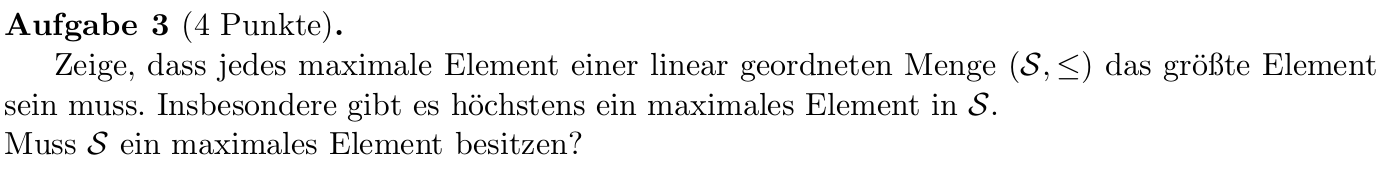
\includegraphics[scale=0.3]{./A-3.png}
        \label{fig:}
    \end{figure}

    \begin{itemize}
        \item a)\\
            \underline{ZZ:} Sei (S,$\leq$) linear geordnet x maximales Element $\Rightarrow$ x größtes Element\\
            \underline{Beweis:}\\
                Sei x maximales Element von S, also gelte:\\
                \\$\nexists y: x < y \Leftrightarrow \forall y: \neg x < y \quad (x \nleq y) \quad \Leftrightarrow \forall y: y \leq x$\\
                \\Wenn  $x \neq y$ folgt mit linearer Ordnung $y < x$\\
                $\Rightarrow x$ ist größtes Element\\

        \item b)\\
            \underline{ZZ:} Sei (S, $\leq$) linear geordnet, dann gibt es höchstens 1 maximales Element\\
            \underline{Beweis:}\\
                Annahme: x und y sind maximale Elemente und $x \neq y$\\
                \\$\Rightarrow \nexists z: x < z$ und $\nexists z: y < z$\\
                $\overset{\text{linear und } x \neq y}{\Rightarrow} x < y \text{ oder } y < x$\\
                Damit gibt es für eines der beiden ein größeres Element.\\

        \item c)\\
            (0,1) hat im offenen Intervall kein maximales Element in $\mathds{R}$\\
    \end{itemize}


%}}}

\section*{}%{{{
\label{sec:aufgabe_4}

    \begin{figure}[H]
        \centering
        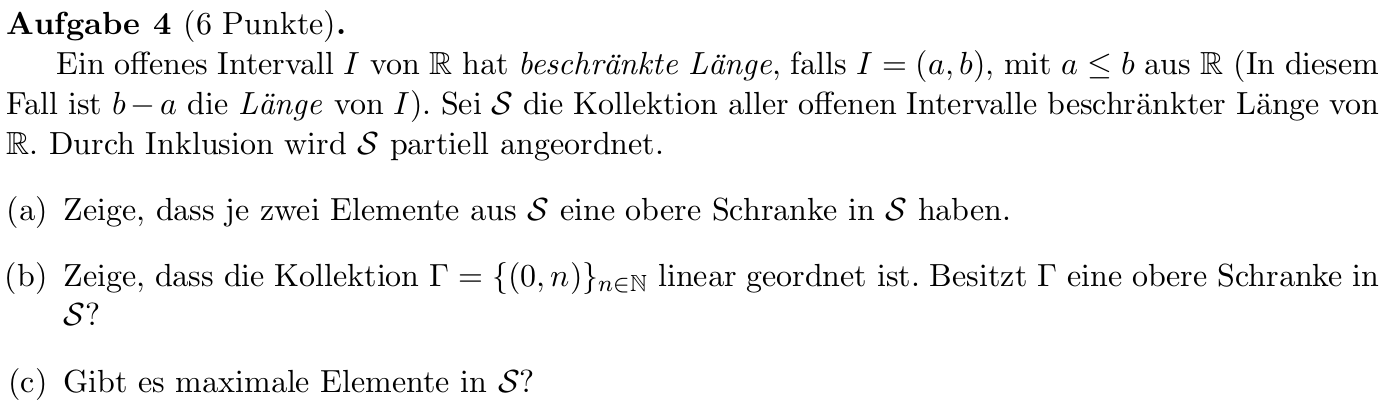
\includegraphics[scale=0.3]{./A-4.png}
        \label{fig:}
    \end{figure}

    \begin{itemize}
        \item a)\\
            \underline{ZZ:} Seien $x,y \in S: \exists z \in S: y \leq z \text{ und } x \leq z$\\
            \underline{Beweis:}\\
                Sei $x = (x_1,x_2), y = (y_1,y_2).$\\
                \\Dann sei $z = (max{x_1,y_1}, max{x_2,y_2})$\\
                $\Rightarrow x \subseteq z$ und $y \subseteq z$\\
                $\Rightarrow x \leq z \text{ und } y \leq z$\\
                $\Rightarrow z$ ist obere Schranke von x und y\\

        \item b)\\
            \begin{itemize}
                \item \underline{ZZ:} $\Gamma = \{0,n\}_{n \in \mathds{N}}$ linear geordnet\\
                    \underline{Beweis:}\\
                    Seien $a,b \in \Gamma$ und $a \neq b \Rightarrow (0,n_a) \neq (0,n_b)$\\
                    $\Leftrightarrow \{0,\dots,n_a\} \subset \{0,\dots,n_b\} \text{ oder } \{0,\dots,n_b\} \subset \{0,\dots,n_a\}$\\
                    $\Leftrightarrow a < b \text{ oder } b < a$\\
                    $\Leftrightarrow \Gamma$ ist linear geordnet

                \item \underline{ZZ:} Es gibt keine obere Schranke\\
                    \underline{Beweis:}\\
                        Annahme: Es gibt eine obere Schranke $B = (0,\dots,b)$\\
                        $\Rightarrow \{0,\dots,n\} \subseteq \{0,\dots,b\}, \forall n \in \mathds{N}$\\
                        $\Rightarrow b > n, \forall n \in \mathds{N}$ Widerspruch!\\
                        \\Es gibt keine obere Schranke.\\

            \end{itemize}

        \item c)\\
            \underline{ZZ:} Es gibt kein maximales Element\\
            \underline{Beweis:}\\
                \begin{itemize}
                    \item Version 1:\\
                        Die Def. des maximalen Elements fordert eine obere Schranke,\\
                        da es keine gibt, gibt es auch kein maximales Element.\\

                    \item Version 2:\\
                        Wenn es ein n = (0,...,n) gibt, gibt es auch immer ein m = (0,...,n+1)\\
                        $\Rightarrow$ es gibt kein Element in $\Gamma$, für dass es kein größeres gibt.\\
                \end{itemize}

    \end{itemize}

%}}}
\end{document}
